\chapter{Users}\label{ch:End-User} 
There are two main types of prosthesis users; persons who are born without a limb, and persons who lost a limb due to trauma or diseases, like diabetes\cite{StrainInjuries}. Some are missing a toe where others have lost an arm or leg, this project will focus on a person with a high-level amputation specifically shoulder disarticulation.\\
    
\section{Shoulder disarticulation}
Users with shoulder disarticulation have their arm amputated at the shoulder. A generalised description of different arm amputations is seen in Figure \ref{fig:Degrees_of_amputations}:

\begin{figure}[H]
    \centering
    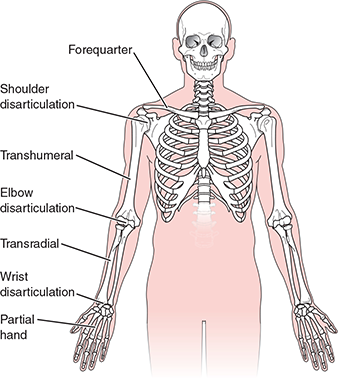
\includegraphics[width=8cm,height=7cm]{Figures/Contextual_figures/Degrees_of_amputation.png}
    \caption{Degrees of arm amputations, including shoulder disarticulation \cite{Disart}}
    \label{fig:Degrees_of_amputations}
\end{figure}
Here the arm is separated at the humerus, the bone that runs from the shoulder to the elbow joint, but the shoulder-socket remains, which leaves some muscle and mobility of the shoulder-joint itself intact.  

\section{Difficulties} \label{Difficoulties}
Loss of limbs creates obstacles on a daily basis. A prosthesis can be a help to minimise these obstacles, assisting the user, so they can function independently and do daily tasks. There are also some difficulties for upper limb amputees who uses prosthesis, some of these is listed bellow.\\

\subsection*{Skin care}
The users residual limb is enclosed in the prosthesis which is sealed airtight around the limb. This leads to sweat not being able to evaporate. The sweat buildup around the limb can result in blisters and irritated skin around the residual limb\cite{SkinCare}.\\

\subsection*{Repetitive Strain Injuries}\\
Physical overloads, caused by the joint of the prosthetic fitting, with pain, as a result, are another well-known issue. Vibrations, rotations and mechanical pressures can amplify the pain.\\
According to research from an Australian survey (1999)  shows that amputees is more likely to get a repetitive strain injury, in fact, the research shows that half of the tested people with prosthesis feels pain while operating repetitive tasks. Here non-amputees reports that only 10 per cent feels the pain \cite{StrainInjuries}.\\

\subsection*{Weight Control}\\
The users' size can fluctuate due to weight, resulting in different sizes on the attachment of the prostheses. If weight is gained, the size of the attachment might get too small, resulting in an imperfect fit causing pain\cite{weightControl}.\\
This project will not focus on making any attachment for the user.

\section{Summary}
The end user of the project is a person with a high level of amputation. Living without a limb creates many difficulties for the individual to overcome.\\
In the next chapter the project looks into which options are available to ease these difficulties and some part-solutions on which systems could be looked at when controlling, e.g. a prosthesis. 